% !TEX root = ./Basilisk-relativeOD-20190620.tex

\section{Model Description}

This module implements a square-root unscented Kalman Filter in order to achieve it's best state estimate of the inertial spacecraft attitude states. The estimated state is spacecraft rotation and velocity in the inertial frame, as well as a bias on the measurements in pixels $\bm b$. 

\textbf{Important:} The default units in Basilisk are meters for distance, and meters per second for speed. These are the units to be used for this filter, though the internals use km and km/s for numerical precision. 

\subsection{Filter Setup} %%%

The equations and algorithm for the square root uKF are given in "inertialUKF$\_$DesignBasis.pdf" [\citenum{Wan2001}] alongside this document.
The filter is therefore derived with the states being $\bm X =\begin{bmatrix} \leftexp{N}{\bm r}&  \leftexp{N}{\bm v}  &  \bm b \end{bmatrix}^{T}$

The dynamics of the filter are given in Equations \eqref{eq:dynInertial}. $\tau$ is the total torque read in by the wheels. 
\begin{align}
\label{eq:dynInertial}
\dot{\bm r} &=\bm v \\
\dot{\bm v} & = - \frac{\mu}{|\bm r|^3} \bm r
\dot{\bm b} & = \bm 0
\end{align}

The propagation is done using an RK4 integrator. 
The following square-root uKF coefficients are used: $\alpha = 0.02$, and $\beta = 2$. 


\subsection{Measurements}

\begin{figure}[H]
	\centerline{
		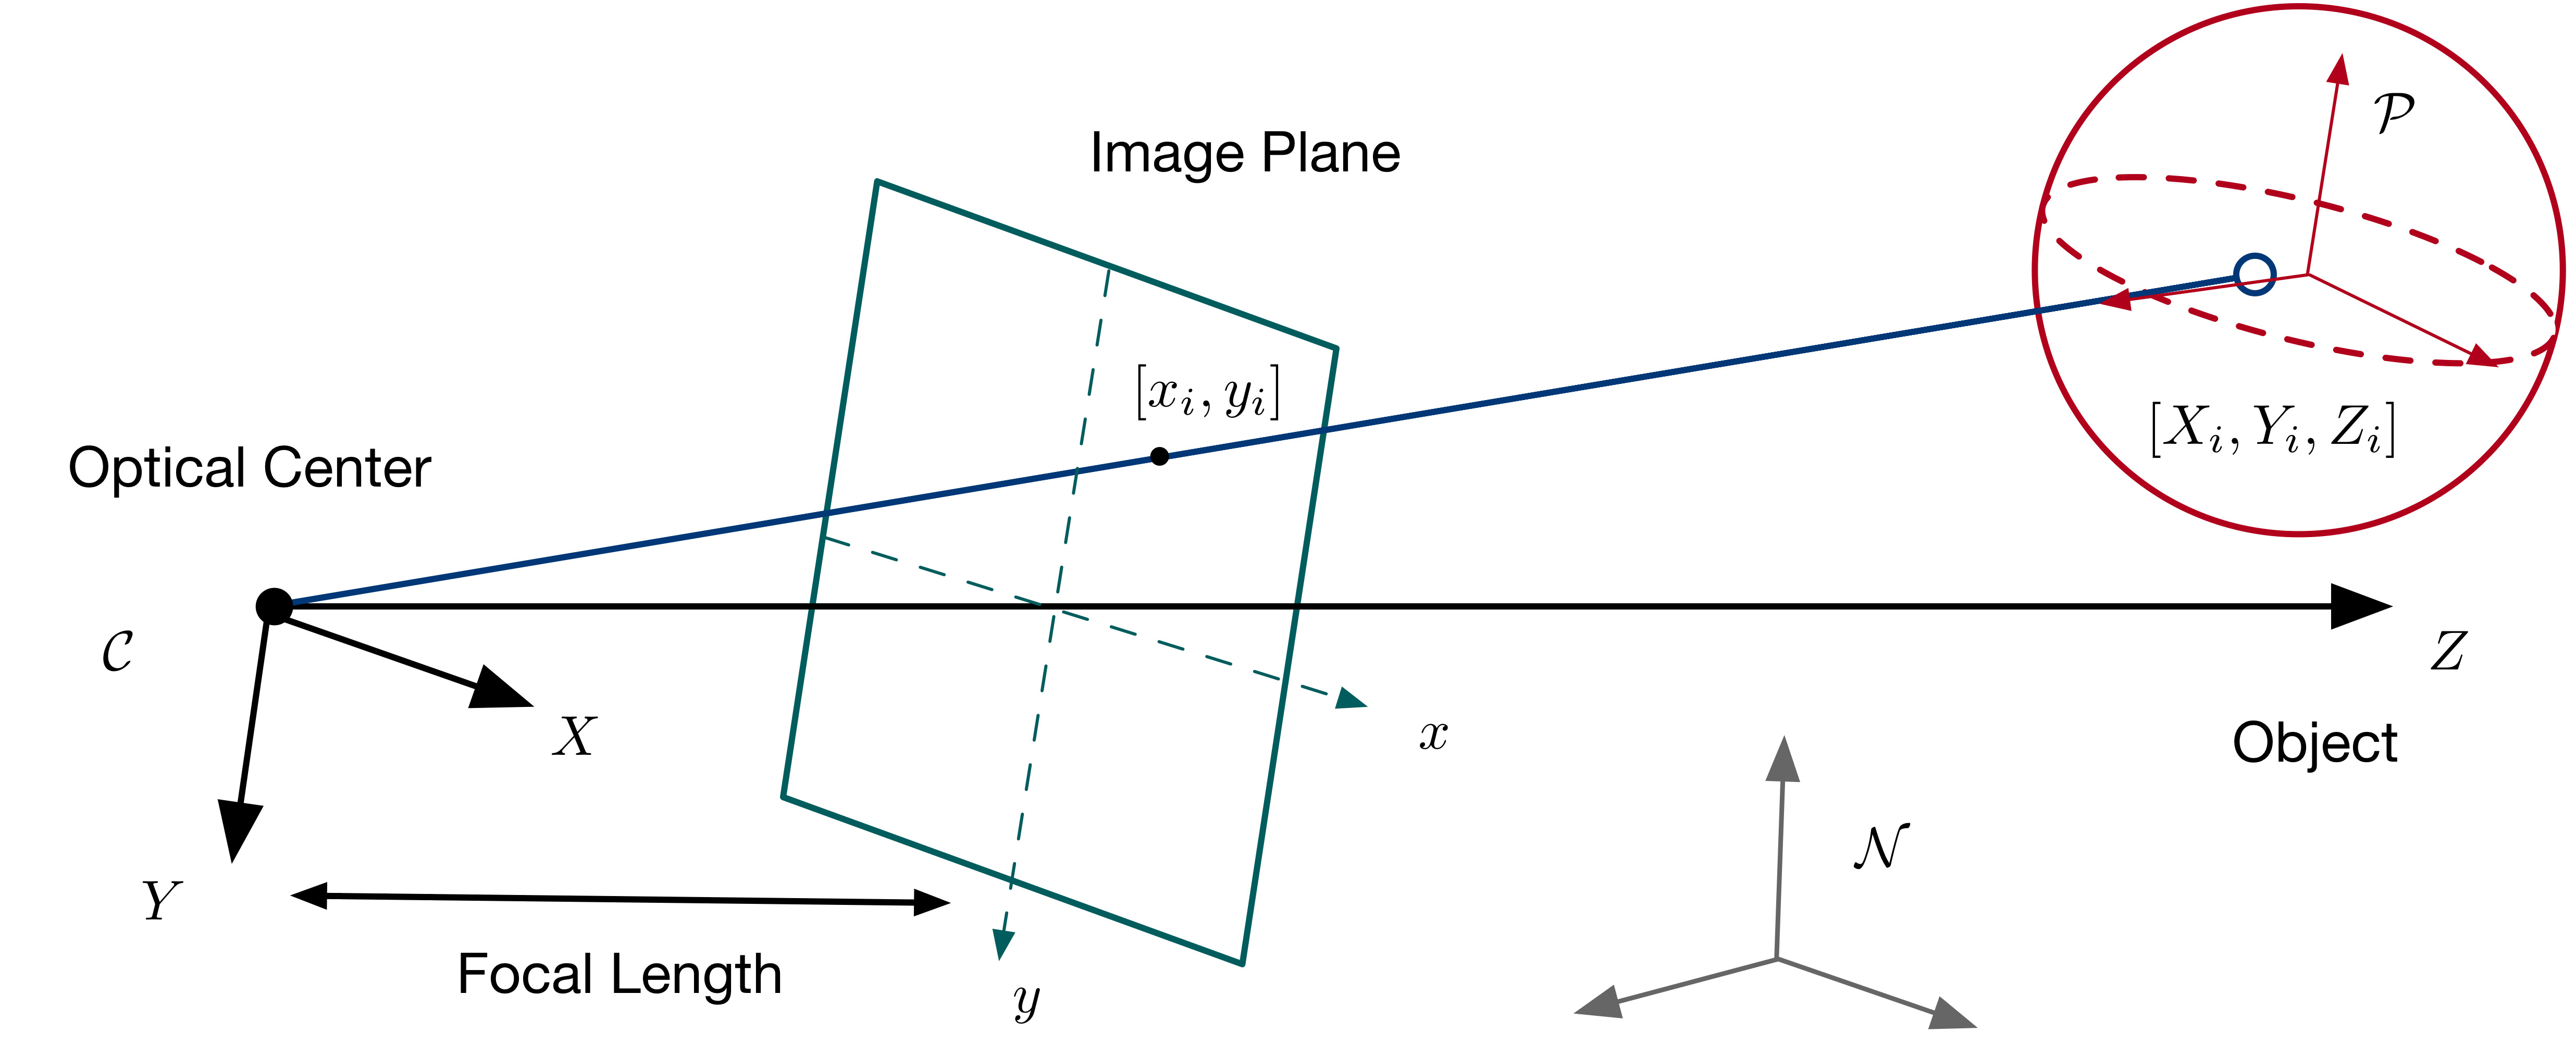
\includegraphics{Figures/CameraGeometry}
	}
	\caption{Camera Model}
	\label{fig:camera}
\end{figure}


This converter module processes the output of a circle finding method to extract spacecraft inertial position. It does this by reading spacecraft attitude (coming from star tracker or other means), camera parameters, and the circle properties. 

Messages read:

\begin{itemize}
\item CameraConfigMsg: containing focal length, resolution, and sensor size. These values are needed for the following computations. Notably the camera frame relative to the body frame is used.
\item CirclesInMsg: Circle radius, center pixel and line, and uncertainty around these values in pixels. 
\item NavAttInMsg: Used for the spacecraft attitude. This allows to move from the body frame to the inertial frame.
\end{itemize}

Message written:
\begin{itemize}
\item OpNavFswMsg: Message containing $\leftexp{N}{\bm r}$ and it's covariance.
\end{itemize}

\subsection{Position computation}

A geometrical method can be used to extract pose information from center and apparent diameter information. The norm of the position vector is given by the apparent size, it's direction is given by the pixel and line data. Using $\leftexp{C}{\bm r_c} = \leftexp{C}{\begin{bmatrix} r_1 & r_2 & r_3 \end{bmatrix}}^T$ as the relative vector of the camera with respect to the celestial center, $A$ as the apparent diameter of the celestial body, $D$ as the actual diameter:

\begin{align}\label{eq:cad}
|\bm r_c| = \frac{1}{2}\frac{D}{\sin\left(\frac{1}{2} A\right)} \hspace{2cm} \frac{1}{r_3}\begin{bmatrix} r_1 \\ r_2 \end{bmatrix}= \frac{1}{r_3}\tilde{\bm r} = \frac{1}{f}\begin{bmatrix} x \\ y \end{bmatrix}
\end{align}

These equations have been used in multiple instances~\cite{Battin, Owen_OpNav}. The third component of $\bm r_c$ provides the range measurement to the body which can be extracted using the apparent diameter measurements. Hence the definition of $\tilde{\bm r}$ which only contains the first two components of $\bm r_c$. The vector components of $\bm r_{c}$ can be expressed relative to the inertial frame assuming inertial attitude knowledge from other instruments. Using the position of the camera on the spacecraft this provides the measurement value for an orbit determination filter using a circle-finding algorithm.  

